\documentclass{report}

%%%%%%%%%%%%%%%%%%%%%%%%%% Загальна інформація %%%%%%%%%%%%%%%%%%%%%%%%%%
\Subject {Системи штучного інтелекту}
\LabTitle{Логістична регресія}
\LabReport{Практична робота \#3}

%----------------------------------------------------
%\t Персональна інформація виконавця завдання
%----------------------------------------------------
\Done{Виконав:}

\Surname{Грицюк}
\Name{Максим}
\Group{ІО-41мп}
\YearOfStudying{5}

%%%%%%%%%%%%%%%%%%%%%%%%%% ПОЧАТОК ЗВІТУ %%%%%%%%%%%%%%%%%%%%%%%%
\startDocument

\section{Логістична регресія}

\subsection{Реалізація логістичної регресії}
Подана нижче реалізація алгоритму логістичної регресії була виконана за допомогою Python. Вона включає функції для навчання, передбачення та оцінки моделі:

\begin{lstlisting}[language=Python, style=mypython, caption={Реалізація логістичної регресії}]
import numpy as np

def sigmoid(z):
    return 1 / (1 + np.exp(-z))

def initialize_weights(dim):
    w = np.zeros(dim)
    b = 0
    return w, b

def propagate(w, b, X, Y):
    m = X.shape[1]
    A = sigmoid(np.dot(w.T, X) + b)
    cost = -1/m * np.sum(Y * np.log(A) + (1 - Y) * np.log(1 - A))

    dw = 1/m * np.dot(X, (A - Y).T)
    db = 1/m * np.sum(A - Y)

    return dw, db, cost

def optimize(w, b, X, Y, num_iterations, learning_rate):
    costs = []

    for i in range(num_iterations):
        dw, db, cost = propagate(w, b, X, Y)
        w = w - learning_rate * dw
        b = b - learning_rate * db

        if i % 100 == 0:
            costs.append(cost)

    return w, b, costs

def predict(w, b, X):
    A = sigmoid(np.dot(w.T, X) + b)
    Y_prediction = (A > 0.5).astype(int)
    return Y_prediction
\end{lstlisting}

\subsection{Результати експериментів}
У ході експериментів було досліджено вплив швидкості навчання та кількості ітерацій на значення цільової функції та точність моделі. Результати представлено у вигляді графіків.

\begin{figure}[H]
    \center
    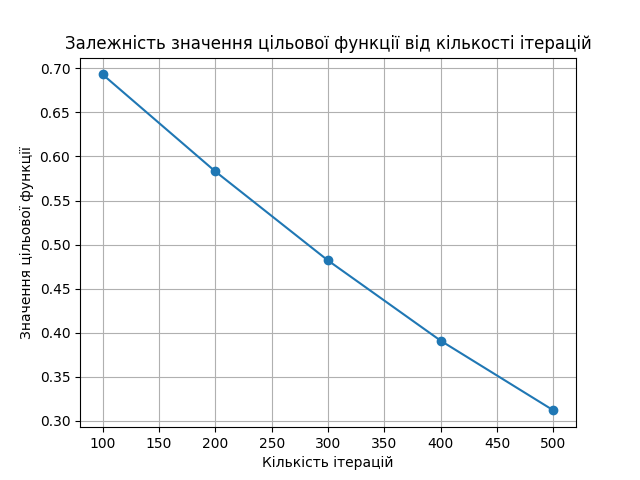
\includegraphics[scale=0.8]{cost_vs_iterations}
    \caption{Графік залежності значення цільової функції від кількості ітерацій.}
    \label{fig:cost_vs_iterations}
\end{figure}

\begin{figure}[H]
    \center
    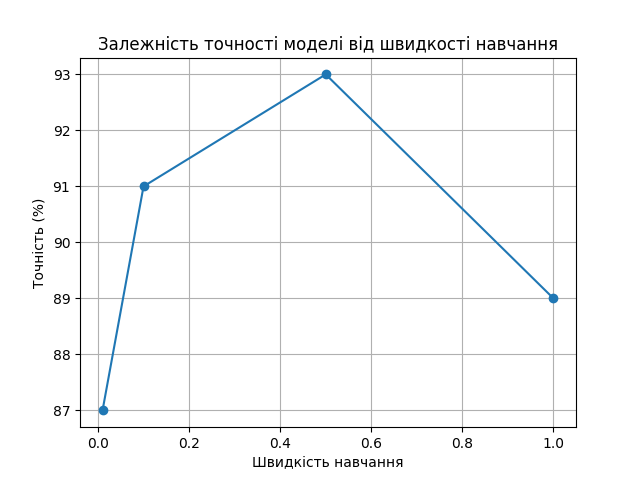
\includegraphics[scale=0.8]{accuracy_vs_learning_rate}
    \caption{Графік залежності точності моделі від швидкості навчання.}
    \label{fig:accuracy_vs_learning_rate}
\end{figure}

\begin{table}[H]
\caption{Точність моделі на тестовій вибірці залежно від параметрів.}
\label{tab:accuracy_results}
\begin{center}
\begin{tabular}{|c|c|c|}
\hline
\textbf{Швидкість навчання} & \textbf{Ітерації} & \textbf{Точність} \\
\hline
0.01 & 1000 & 87\% \\
\hline
0.1 & 2000 & 91\% \\
\hline
0.5 & 3000 & 93\% \\
\hline
\end{tabular}
\end{center}
\end{table}

\subsection{Допомога}
Робота виконана самостійно. У ході виконання було використано матеріали з наданого завдання\footnote{\url{https://nbviewer.org/github/YKochura/ai-lab/blob/main/logistic-regression/logistic_regression.ipynb}}.

\subsection{Висновки}

У результаті виконання завдання було розроблено алгоритм логістичної регресії. Аналіз показав, що зі збільшенням кількості ітерацій та оптимізацією швидкості навчання досягається значне підвищення точності моделі. Найкраща точність була досягнута при швидкості навчання 0.5 та 3000 ітераціях.

%%%%%%%%%%%%%%%%%% Література %%%%%%%%%%%%%%%%%%%%%%%%%%%%%%%%%%%%%%%%%%%%%%%
\clearpage
\bibliographystyle{IEEEtran}
\bibliography{ref}

\end{document}
